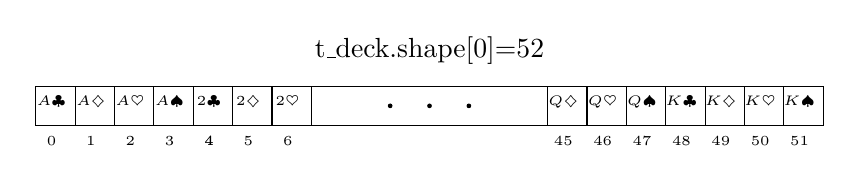
\begin{tikzpicture}
    % Define grid dimensions
    \def\n{1} % N = 5 rows
    \def\m{20} % M = 5 columns
    \def\cellsize{0.5} % Size of each cell

    % Draw the grid
    \foreach \i in {0,...,\n} {
        \draw[black] (0,\i*\cellsize) -- (\m*\cellsize,\i*\cellsize); % Horizontal lines
    }
    % \foreach \j in {0,...,\m} {
    %     \draw[black] (\j*\cellsize,0) -- (\j*\cellsize,\n*\cellsize); % Vertical lines
    % }

    Place dots in the middle row (row 3, columns 2, 3, and 4)
    \foreach \j in {0,1,2} {
        \fill[black] ({(1-\j)/2+\m*\cellsize/2}, 0.5*\cellsize) circle (0.03); % Dots
    }

    \foreach \j in {0,...,\m} {
        \ifnum\j<8 % Check if j < 10
            \draw[black] (\j*\cellsize,0) -- (\j*\cellsize,\n*\cellsize); % Draw line
        \else
            \ifnum\j>12 % Check if j > 20
                \draw[black] (\j*\cellsize,0) -- (\j*\cellsize,\n*\cellsize); % Draw line
            \fi
        \fi
        }

    % Draw the outer rectangle
    \draw[black] (0,0) rectangle (\m*\cellsize, \n*\cellsize);

    % Add the shape label below the grid
    \node[below] at ({\m/2*\cellsize}, 2.5*\cellsize) {\pyvar{t\_{deck}.shape[0]=52}};

    % \draw[->, thin, decorate, decoration={coil, segment length=7mm, amplitude=2mm}] 
    %     ({(\m-2)*\cellsize+0.1}, \n*\cellsize+0.1) -- ++(2,1) % Arrow starts at (5,5) and extends 2 units right
    %     node[above, right, align=left] {\small A card has \\ \;$\cdot$ a rank\\ \;$\cdot$ a suit}; % Text at the end of the arrow

    \node at (0.4*\cellsize, \n*\cellsize-0.4*\cellsize) {\tiny $A\clubsuit$};
    \node at (1.4*\cellsize, \n*\cellsize-0.4*\cellsize) {\tiny $A\diamondsuit$};
    \node at (2.4*\cellsize, \n*\cellsize-0.4*\cellsize) {\tiny $A\heartsuit$};
    \node at (3.4*\cellsize, \n*\cellsize-0.4*\cellsize) {\tiny $A\spadesuit$};
    \node at (4.4*\cellsize, \n*\cellsize-0.4*\cellsize) {\tiny $2\clubsuit$};
    \node at (5.4*\cellsize, \n*\cellsize-0.4*\cellsize) {\tiny $2\diamondsuit$};
    \node at (6.4*\cellsize, \n*\cellsize-0.4*\cellsize) {\tiny $2\heartsuit$};

    \node at (13.4*\cellsize, \n*\cellsize-0.4*\cellsize) {\tiny $Q\diamondsuit$};
    \node at (14.4*\cellsize, \n*\cellsize-0.4*\cellsize) {\tiny $Q\heartsuit$};
    \node at (15.4*\cellsize, \n*\cellsize-0.4*\cellsize) {\tiny $Q\spadesuit$};
    \node at (16.4*\cellsize, \n*\cellsize-0.4*\cellsize) {\tiny $K\clubsuit$};
    \node at (17.4*\cellsize, \n*\cellsize-0.4*\cellsize) {\tiny $K\diamondsuit$};
    \node at (18.4*\cellsize, \n*\cellsize-0.4*\cellsize) {\tiny $K\heartsuit$};
    \node at (19.4*\cellsize, \n*\cellsize-0.4*\cellsize) {\tiny $K\spadesuit$};
    \node at (0.4*\cellsize, \n*\cellsize-1.4*\cellsize) {\tiny 0};
    \node at (1.4*\cellsize, \n*\cellsize-1.4*\cellsize) {\tiny 1};
    \node at (2.4*\cellsize, \n*\cellsize-1.4*\cellsize) {\tiny 2};
    \node at (3.4*\cellsize, \n*\cellsize-1.4*\cellsize) {\tiny 3};
    \node at (4.4*\cellsize, \n*\cellsize-1.4*\cellsize) {\tiny 4};
    \node at (4.4*\cellsize, \n*\cellsize-1.4*\cellsize) {\tiny 4};
    \node at (5  .4*\cellsize, \n*\cellsize-1.4*\cellsize) {\tiny 5};
    \node at (6.4*\cellsize, \n*\cellsize-1.4*\cellsize) {\tiny 6};

    \node at (13.4*\cellsize, \n*\cellsize-1.4*\cellsize) {\tiny 45};
    \node at (14.4*\cellsize, \n*\cellsize-1.4*\cellsize) {\tiny 46};
    \node at (15.4*\cellsize, \n*\cellsize-1.4*\cellsize) {\tiny 47};
    \node at (16.4*\cellsize, \n*\cellsize-1.4*\cellsize) {\tiny 48};
    \node at (17.4*\cellsize, \n*\cellsize-1.4*\cellsize) {\tiny 49};
    \node at (18.4*\cellsize, \n*\cellsize-1.4*\cellsize) {\tiny 50};
    \node at (19.4*\cellsize, \n*\cellsize-1.4*\cellsize) {\tiny 51};
    
\end{tikzpicture}
